\chapter{XEMC: A Package for Inclusive Cross Section Models}

\section{Overview}
 XEMC is a stand-alone package written in C++ to calculate the inclusive cross section of electron-nucleus scattering. It is composed of three cross section models for the inelastic (DIS) process, three cross section models for the quasi-elastic (QE) process, and a radiative correction (RC) subroutine based on the peak approximation. In this model, the Born cross section ($\mathrm{\sigma^{Born}_{model}}$) is the sum of the inelastic cross section ($\mathrm{\sigma^{DIS}_{model}}$) and the QE cross section ($\mathrm{\sigma^{QE}_{model}})$. The RC subroutine calculates the radiative cross section ($\mathrm{\sigma^{rad}_{model}}$) from the Born cross section. The parameters of kinematic settings and target configurations are all defined in an external file.
 
 Cross section models are usually developed based on theoretical calculations, world data and additional corrections. Different models are designed for specific kinematic regions, depending on the physics processes and the final states. The inclusive cross section measured by the E08-014 was above the QE peak and can be well modelled by the y-scaling~\cite{West1975263,PhysRevC.41.R2474,Boffi19931,john_thesis}. The QE model was further iterated through comparing with experimental data at the similar kinematics. The DIS contribution to the total cross section was small and was calculated with the most updated DIS model~\cite{Bosted:2012qc}. 
  
  The basic structure of the package will be briefly introduced here, followed by a discussion of the cross section models. The results calculated with this code will be compared with experiment results. And a simple example of how to use this code is also given in the end. 
  
\section{Code Structure}
\begin{figure}[!ht]
 \begin{center}
  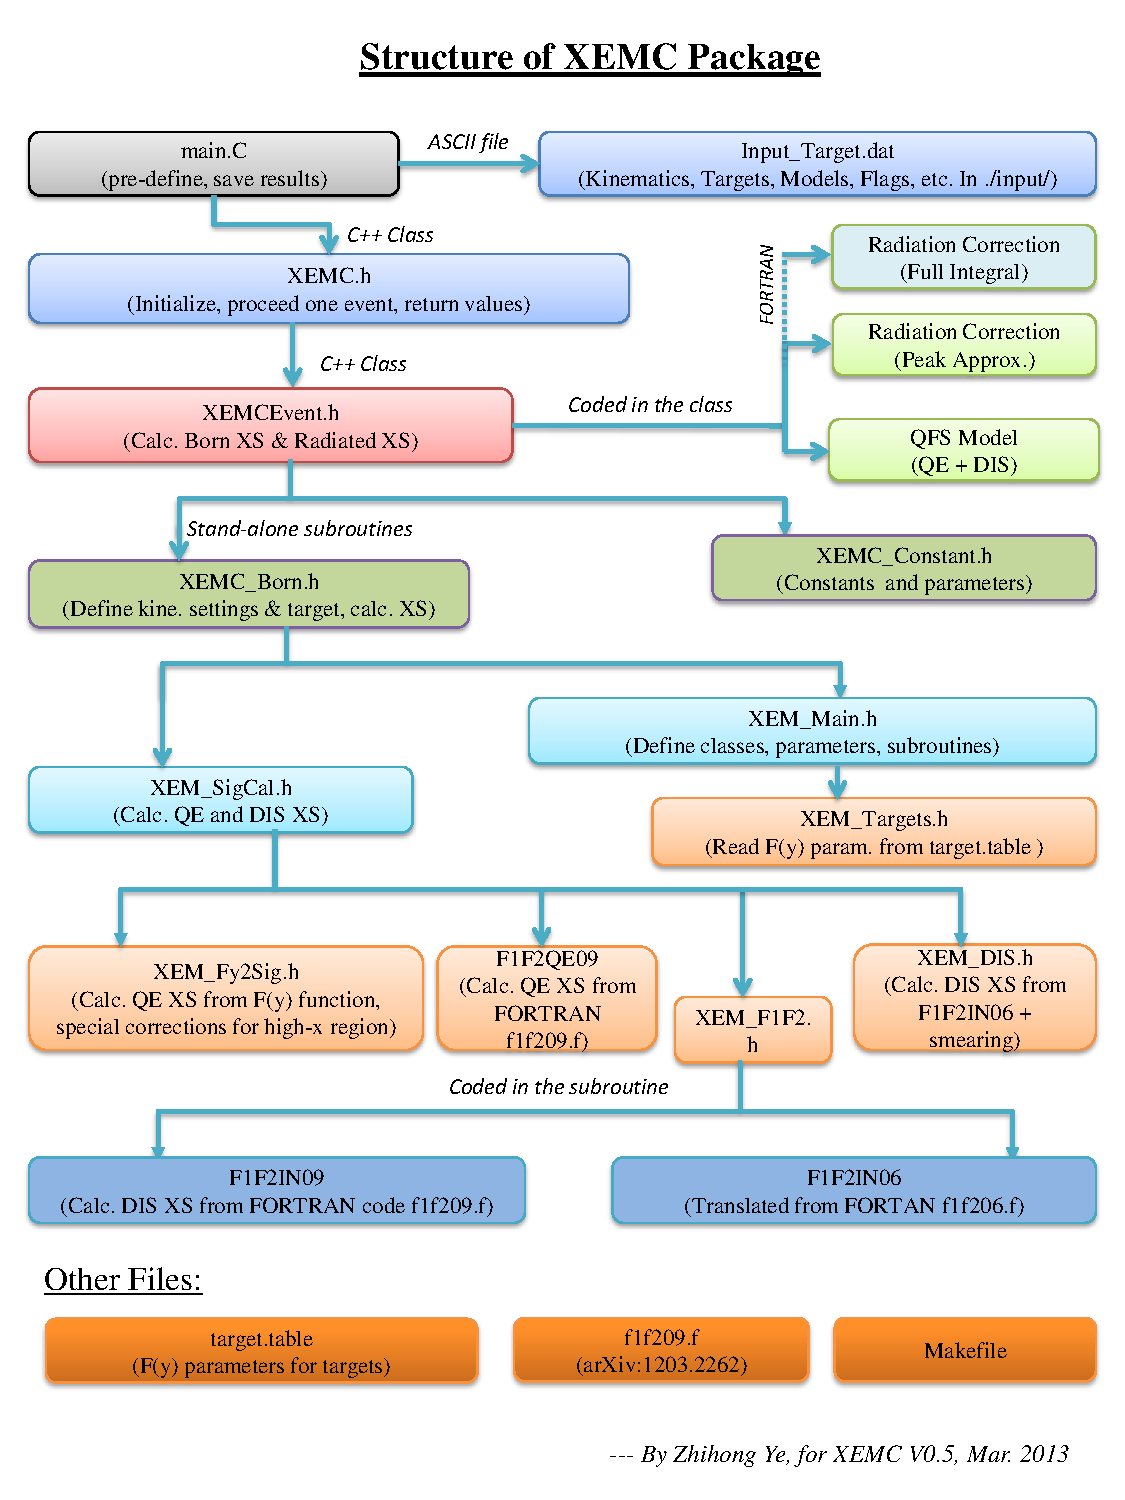
\includegraphics[angle=0,width=1.0\textwidth]{./figures/xemc/XEMC_Structure}
  \caption[Structure of XEMC package]{Structure of XEMC package}
  \label{xemc_struct}
 \end{center}
\end{figure}
\begin{figure}[!ht]
 \begin{center}
  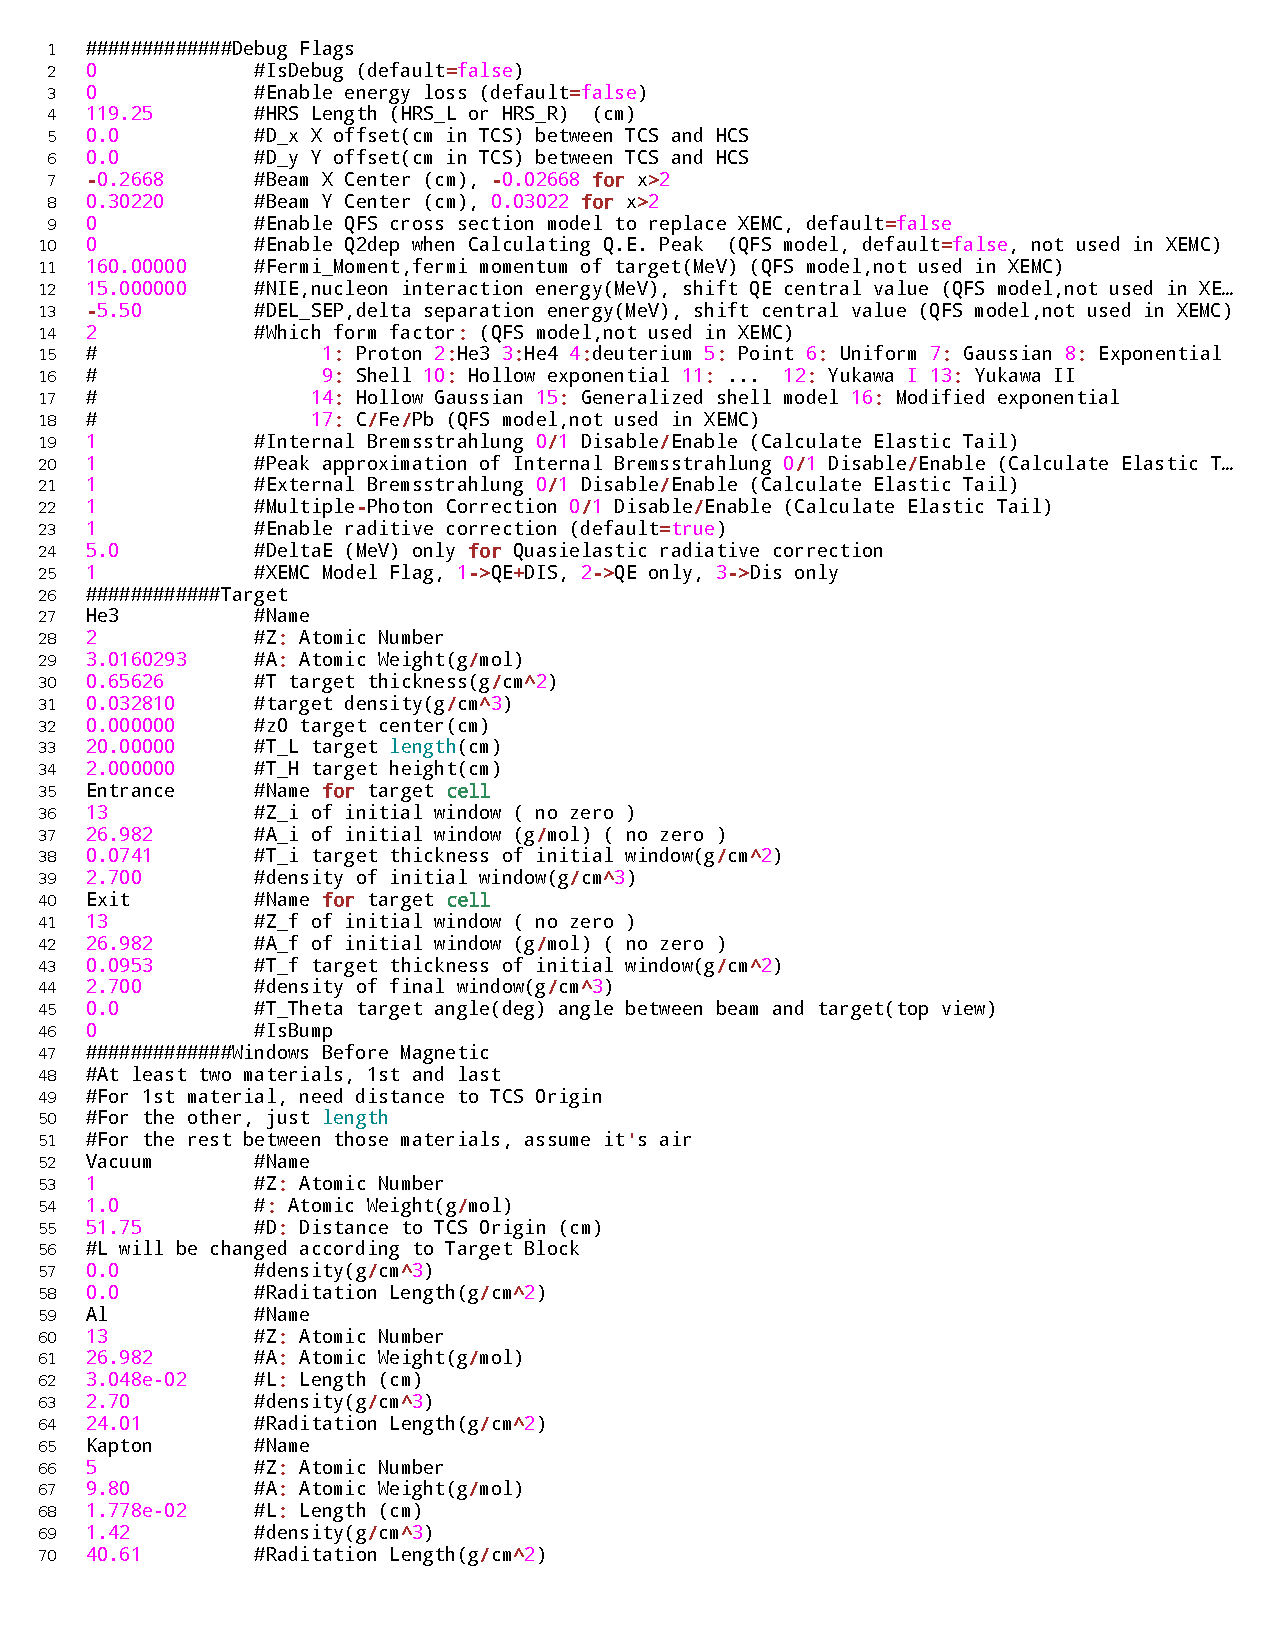
\includegraphics[angle=0,width=1.01\textwidth]{./figures/xemc/He3_Input}
 \caption[Input file for $\mathrm{^{3}He}$ target]{Input file for $\mathrm{^{3}He}$ target}
 \label{xemc_tgt_he3}
 \end{center}
\end{figure} 
Fig.~\ref{xemc_struct} shows the basic structure of the XEMC package. Outside the main code, the input file (Fig.~\ref{xemc_tgt_he3}) is defined to specify the choice of cross section models and any additional physics processes, such as the radiative correction. The reaction location can be corrected by giving the spectrometer center offset and beam position offset. The input file also includes the configuration of the target system, i.e. the target's name, mass and thickness. For cryo-targets, the materials of the target cell, the entrance and the exit of the target chamber are also given. Parameters in the input file are initialized only once in the code.

  A XEMC event has its specified values of the initial and scattered energies as well as the scattering angle. The Born cross section and radiated cross section of this event are calculated in \emph{XEMCEvent.h} where the QFS model is embedded by default.  Other Born cross section models are stored in an independent subroutine, \emph{$\mathrm{XEMC\_Born.h}$}, which will be introduced in next few sections. Once the target configuration and the kinematic setting are pre-defined, the RC subroutine in \emph{XEMCEvent.h} begins to calculate the radiated cross section. 

\section{Quasi-Elastic Cross Section Models}
 Three different QE cross section models, QE-XEM, QE-QFS, and QE-F1F209, are coded in this package. Each model will be introduced below.

 \subsection{QE-XEM} 
  \begin{figure}[!ht]
 \begin{center}
  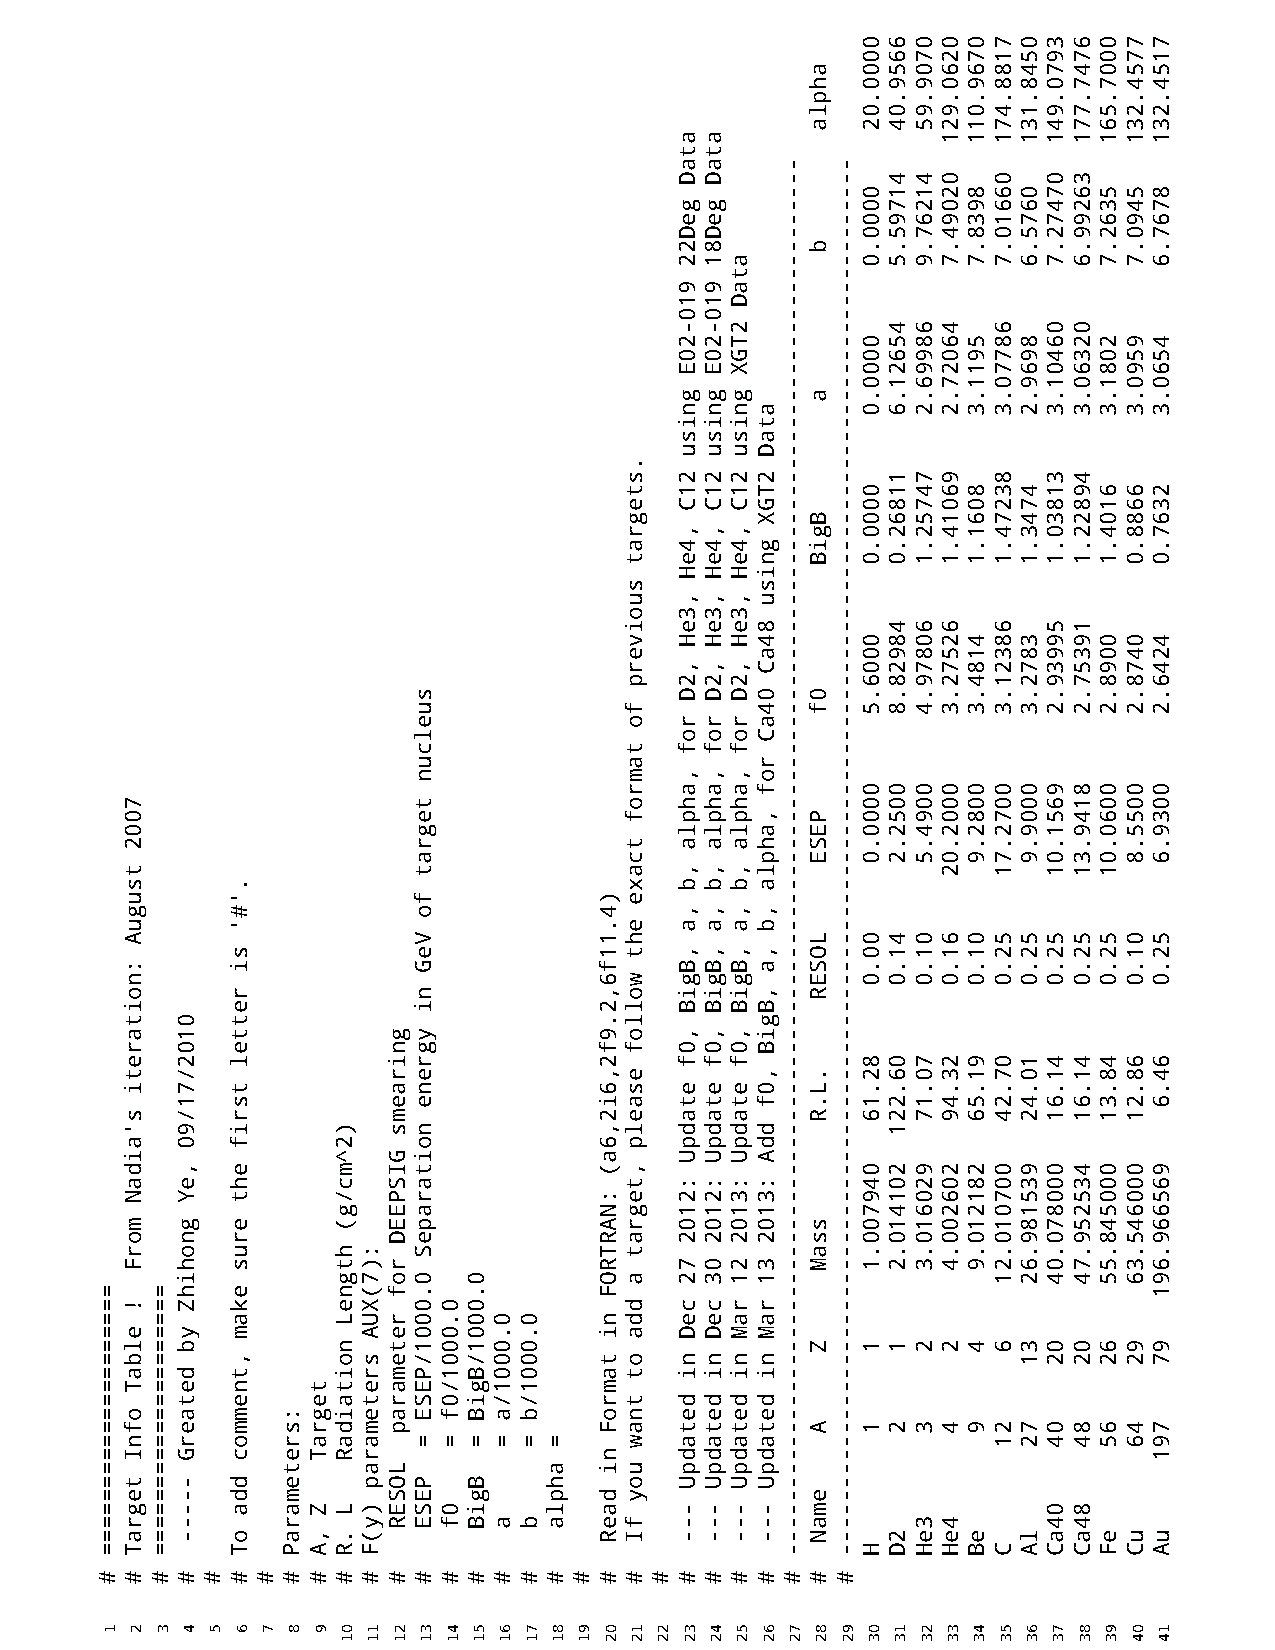
\includegraphics[angle=0,width=1.0\textwidth]{./figures/xemc/target_table}
  \caption[F(y) parameters for a list of targets]{F(y) parameters for a list of target. The file is called target.table which is in ASCII format. The values had been refitted with cross section results from the E02-019 and the E08-014. These values could be changed in the future.}
  \label{xemc_tgt_table}
 \end{center}
\end{figure} 

 QE-XEM was converted from the XEM cross section model, a FORTRAN package developed by the EMC collaboration in Hall-C at JLab~\cite{nadia_thesis,aji_thesis}. XEM includes a QE model (QE-XEM) based on y-scaling~\cite{West1975263,PhysRevC.41.R2474,Boffi19931,john_thesis}, a DIS model (DIS-XEM, see next section), and a RC subroutine. The entire subroutines have been converted into C++ (except the RC part) and coded in \emph{$XEMC\_Born.h$}. QE-XEM is the default QE model in the package.
 
  The scaling function, F(y) (Eq.~\eqref{fy_scaling_eq2} in Section 1.2.2), is directly fitted from experimental data. F(y) for $\mathrm{^{2}H}$ can be extracted from the function~\cite{PhysRevLett.56.1452}:
  \begin{equation}
  F(y) = (f_{0}-B)\frac{\alpha^{2}e^{-(\alpha y)^{2}}}{\alpha^{2}+y^{2}} + B e^{-b|y|},
  \label{fy_fit_func1}
  \end{equation}
where, $f_{0}$, $B$, $\alpha$, $a$ and $b$ are the parameters corresponding to the target. For heavy targets, the second term in the formula above is different:
  \begin{equation}
  F(y) = (f_{0}-B)\frac{\alpha^{2}e^{-(\alpha y)^{2}}}{\alpha^{2}+y^{2}} + B e^{-(by)^{2}}.
    \label{fy_fit_func2}
  \end{equation}

  For a list of targets, the parameters of $F(y)$ function ($f_{},~B,~\alpha,~a,~and~b$) are stored in an external ASCII file, called \emph{target.table}. To extract the parameters, one needs to  obtain the distribution of $F(y)$ from the experimental cross sections:
  \begin{equation}
   F(y) = \sigma_{EX}^{QE}\cdot\frac{1}{Z\sigma_{p}+N\sigma_{n}}\frac{q}{\sqrt{M^{2}+(y+q)^{2}}},
  \end{equation}
where $q=\sqrt{Q^{2}+\nu^{2}}$, and $y$ is the solution of the equation:
\begin{equation}
  M_{A}+\nu = \sqrt{M^{2}+q^{2}+y^{2}+2yq}+\sqrt{M_{A-1}^{2}+y^{2}},
\end{equation}
where $M$ is the mass of the struck nucleon, $M_{A}$ and $M_{A-1}$ are the masses of the target nucleus and the mass of the recoil system, respectively.

 The experimental QE cross sections, $\sigma_{EX}^{QE}$, can be extracted from the experimental Born cross sections subtracted by the DIS cross sections calculated from the model, i.e. $\sigma_{EX}^{QE}=\sigma_{EX}^{Born}-\sigma_{model}^{DIS}$. Hence, different DIS models yield different fitting values of the F(y) parameters. Fig.~\ref{xemc_tgt_table} gives a target table which lists the values of these parameters for all measured targets. The parameters have been determined from the the E02-019~\cite{nadia_thesis} and the E08-014 data with the DIS model, DIS-F1F209 (discussed in Section B.4.3). 
 
 \subsection{QE-QFS}
  QE-QFS is based on the QFS model, a phenomenological model~\cite{qfs_org,qfs_note} which has been used since 1960s. The model was designed to calculate both QE and DIS cross sections with the Plane-Wave Impulse Approximation (PWIA) and it works well at lower $Q^{2}$ region. The complete description of the QFS model can be found in Ref.~\cite{qfs_org,qfs_org2}. The subroutines of the model are coded in $XEMCEvent.h$ and were originally developed and maintained by the collaboration from Temple University~\cite{karl_thesis, hyao_thesis,whita}. 
   
 \subsection{QE-F1F209}
 QE-F1F209 is a part of the cross section model, F1F2QE09, which was developed by P. Bosted and V. Mamyan~\cite{Bosted:2012qc} based their work on empirical fit to electron-nucleus scattering. The model is coded in a stand-alone FORTRAN program, \emph{f1f209.f}. An external link is given in the XEMC package to call the subroutines in the FORTRAN code. To successfully compile the code, a library named \emph{libg2c.so} must be specified in the \emph{Makefile}.
 
\section{DIS Models}
 The DIS cross section model not only calculates the cross section of the deep inelastic scattering process but also includes other inelastic processes, such as resonance productions. There are three DIS models coded in the package. Since the kinematic settings of the E08-014 was well above the QE peak, the contribution from inelastic processes is relatively small, and these models were not iterated with the existing DIS data. 
 
\subsection{DIS-QFS}
 DIS-QFS is a part of the QFS subroutines~\cite{hyao_thesis}.  This model includes the following processes:
 \begin{itemize}
  \item Scattering from two interacting nucleons (MEC in Dip region between the QE peak and the resonances),
  \item Delta Electroproduction ($\Delta$),
  \item Resonance productions at 1500~MeV and 1700~MeV, and,
  \item Deep inelastic scattering (DIS).
 \end{itemize}
  
\subsection{DIS-XEM}
 DIS-XEM was specially designed for the XEM experiment based on P. Bosted's previous empirical fit, F1F2IN06~\cite{Bosted:2006}. To agree with the EMC data, the model included several corrections in different range of $0.8<x_{bj}<1.0$ , and the code became complicated and runs slowly, especially when performing radiative correction. The subroutines have been converted from FORTRAN into C++ and coded in \emph{$XEMC\_Born.h$}. 

\subsection{DIS-F1F209}
 DIS-F1F209 comes from F1F2IN09 and is coded in $f1f209.f$. It is the default DIS model in XEMC.

\section{Radiative Corrections}
\begin{figure}[!ht]
 \begin{center}
  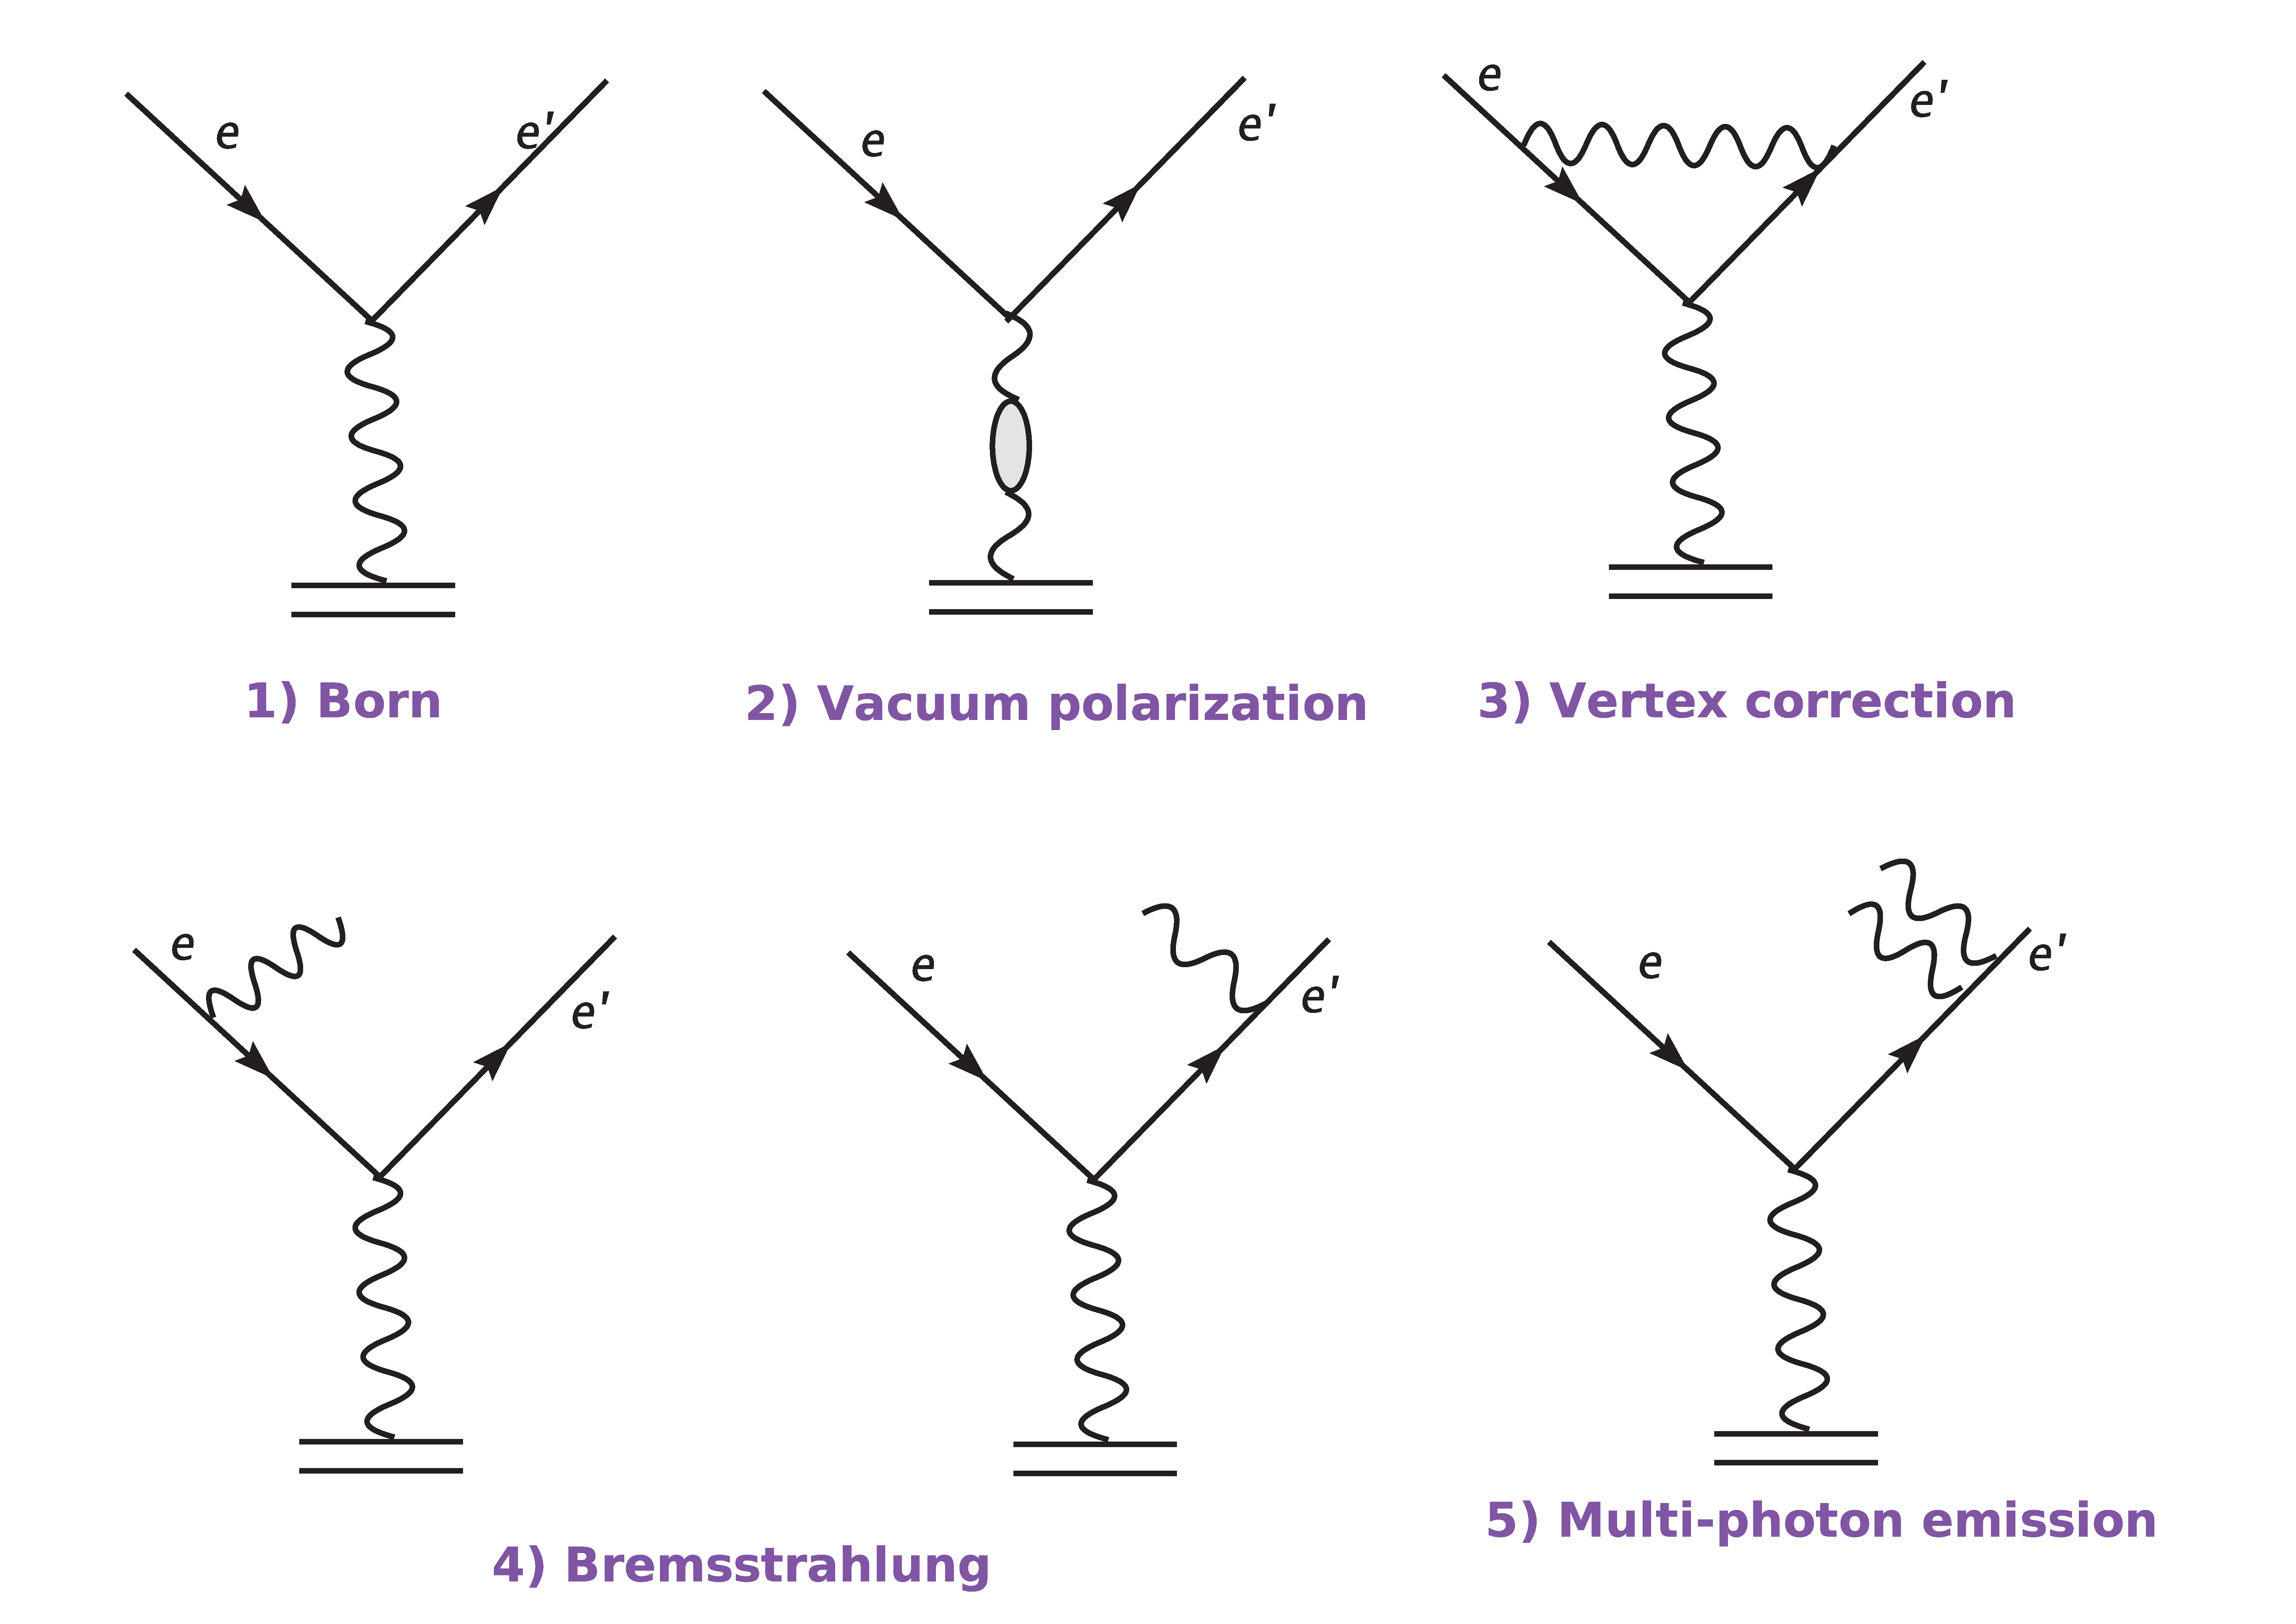
\includegraphics[angle=0,width=0.8\textwidth]{./figures/physics/radiated_feymann}
  \caption[Feynman diagrams for radiation effect]{Feynman diagrams for radiation effect in inclusive lepton-nucleon scattering. Only the lowest orders are shown here.}
  \label{rad_feynm}
 \end{center}
\end{figure} 
 The electron-nucleon scattering process can be modelled by one-photon-exchange-approximation (OPEA), where the electron and the nucleon interact by exchanging one virtual photon. The inclusive cross section of the process is called the Born cross section. There are higher order processes, called radiative effects, contributing to the measured cross sections, as shown in Fig.~\ref{rad_feynm}. The experimental raw cross section is named as the radiated cross section, which has to be corrected to obtain the experimental Born cross section: 
 \begin{equation}
  \sigma^{EX}_{Born} = \frac{\sigma^{Model}_{Born}}{\sigma^{Model}_{rad}}\cdot\sigma^{EX}_{rad},
 \end{equation}
where $\sigma^{Model}_{Born}$ and $\sigma^{Model}_{rad}$ are the Born and radiated cross section calculated from the model, while $\sigma^{EX}_{Born}$ and $\sigma^{EX}_{rad}$ are the Born and radiated cross sections measured from the experiment. The ratio term is generally called the radiative correction factor. 
 
  The radiation effects contain the external radiation and the internal radiation. The external radiation, including external bremsstrahlung and ionization, happens when the incoming or the outgoing electron radiates a real photon when it interacts with the nuclear medium other than the target nucleon. This effect mainly depends on the material and thickness of the target. The internal radiation contains the soft processes, such as internal bremsstrahlung, and the hard processes, such as vacuum polarization, vertex corrections and multiple-photon exchange. The initial and final energies of the electron are modified during those processes, which causes the measured cross section to deviate from the Born cross section.

   The idea of radiative correction is carefully discussed in~\cite{mo_sai_rad, stein_radiation}, and a radiative correction package, RadCor, was developed based on this idea~\cite{karl_thesis,hyao_thesis}. Peak approximation method was used in the package to reduce the CPU time of the radiated cross section calculation. Important subroutines in this package have been migrated to XEMC. 
   
 \section{Performance} 
  In this section, the cross sections calculated from XEMC with the QE-XEM model and the DIS-F1F209 model are directly compared with previous experiment data stored in the QES-Archive~\cite{qe_donal} (Fig.~\ref{xs_achieve_com1} and Fig.~\ref{xs_achieve_com2}) as well as the E02-019 data (Fig.~\ref{xs_nadia_b1} and Fig.~\ref{xs_nadia_b2}). Overall, the model and the data agree nicely. The performance of the radiative correction was examined with the E02-019 data of which the target configurations were known. From Fig.~\ref{xs_nadia_r1} and Fig.~\ref{xs_nadia_r2}, the radiated cross sections from XEMC agree well with the data above the QE region. At $x_{bj}<1$ a small deviation can be seen due to the use of the peak approximation method. The E08-014 data is well above the QE peak so the deviation wasn't important. 
\begin{figure}[!h]
  \begin{center}
    \subfloat[$\mathrm{^{2}D}$ from Arrington 1995]{
      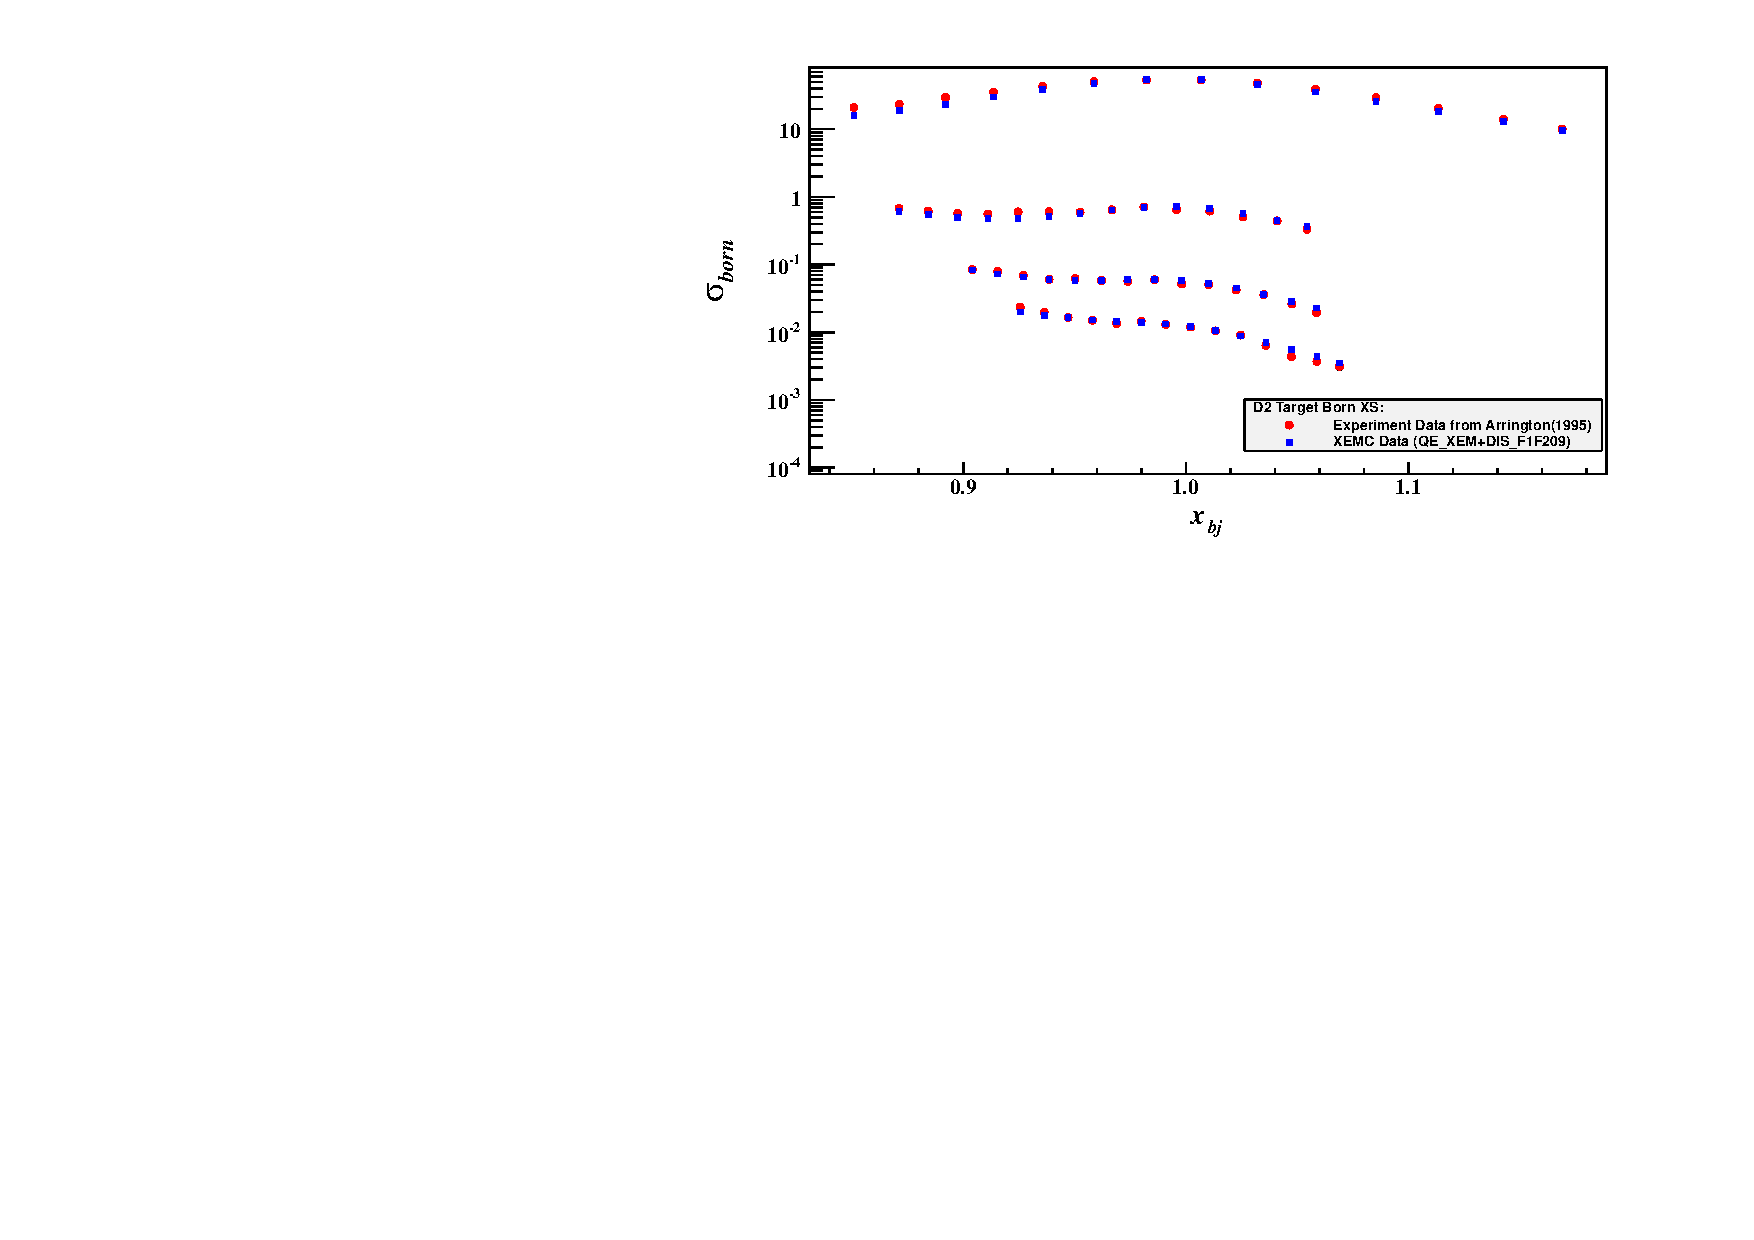
\includegraphics[type=pdf,ext=.pdf,read=.pdf,width=0.9\textwidth]{./figures/xemc/QEA_D2_Jan16_Born_Com_Arrington_1995}
    }
    \\
     \subfloat[$\mathrm{^{3}He}$ from Day 1979]{
      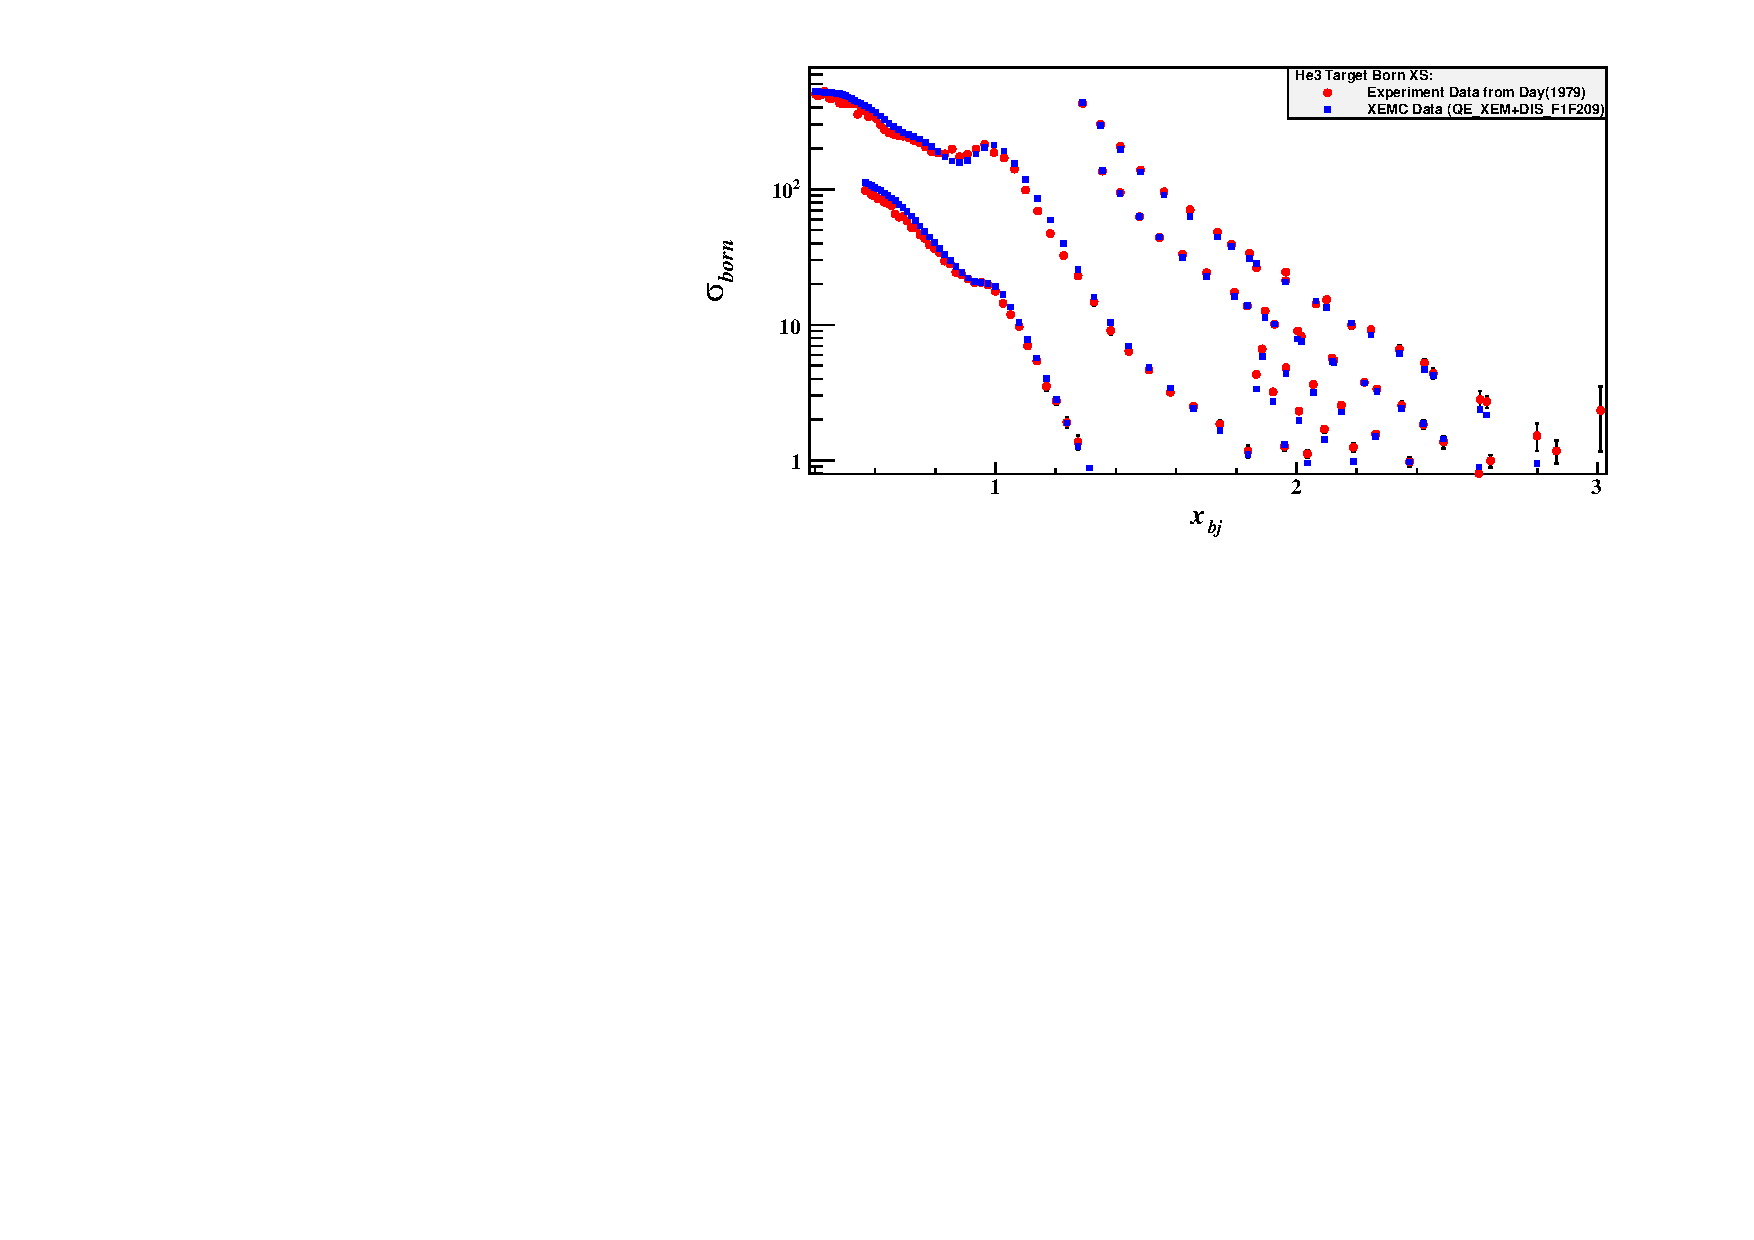
\includegraphics[type=pdf,ext=.pdf,read=.pdf,width=0.8\textwidth]{./figures/xemc/QEA_He3_Jan16_Born_Com_Day_1979}
    }
     \caption[Comparing XEMC models and experiment data for $\mathrm{^{2}D}$ and $\mathrm{^{3}He}$]{\footnotesize{Comparing XEMC models and experiment data for $\mathrm{^{2}D}$ and $\mathrm{^{3}He}$. Data is from QES-Archive~\cite{qe_donal}.}}
    \label{xs_achieve_com1}
  \end{center}
\end{figure}
\begin{figure}[!h]
  \begin{center}
     \subfloat[$\mathrm{^{4}He}$ from Meziani 1992]{
      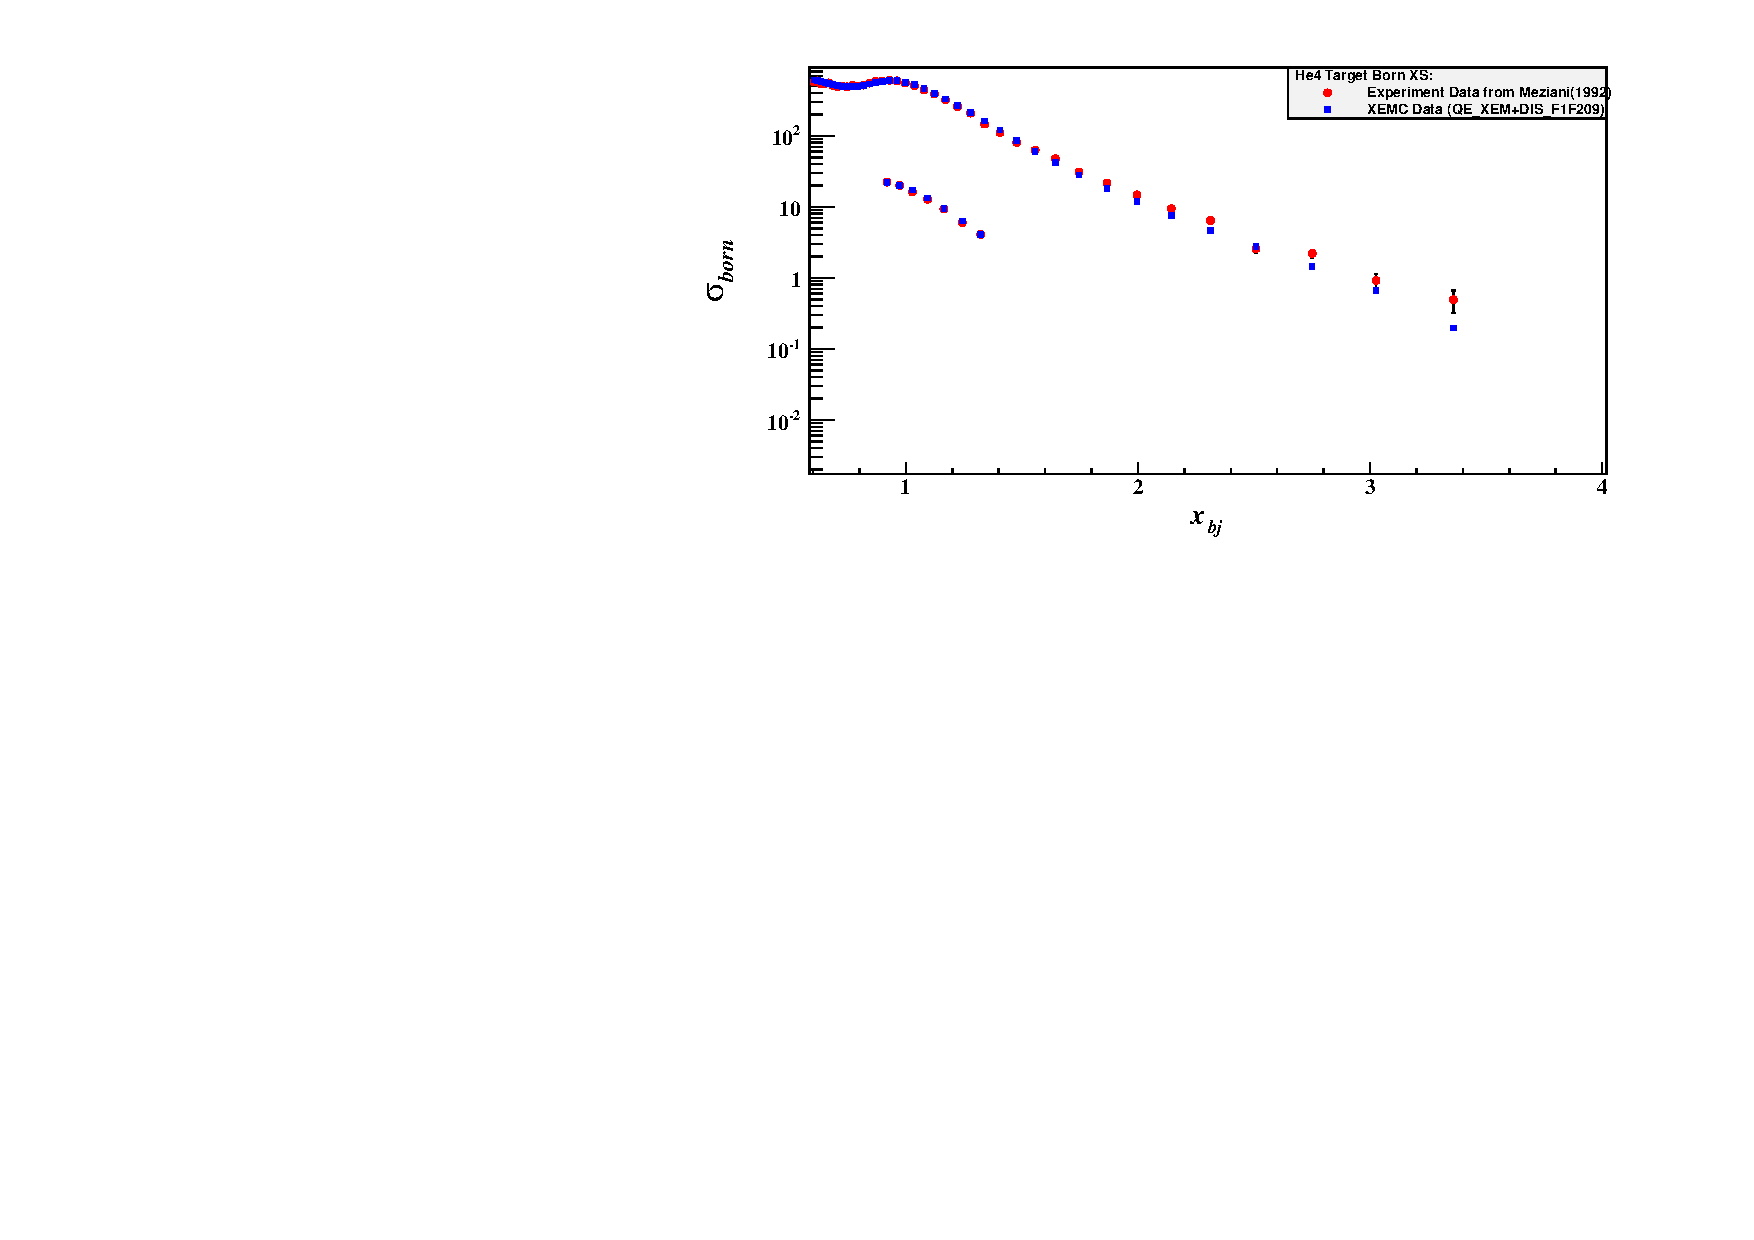
\includegraphics[type=pdf,ext=.pdf,read=.pdf,width=0.9\textwidth]{./figures/xemc/QEA_He4_Jan16_Born_Com_Meziani_1992}
      \label{target_run1}
    }
    \\
     \subfloat[$\mathrm{^{12}C}$ from Arrington 1998]{
      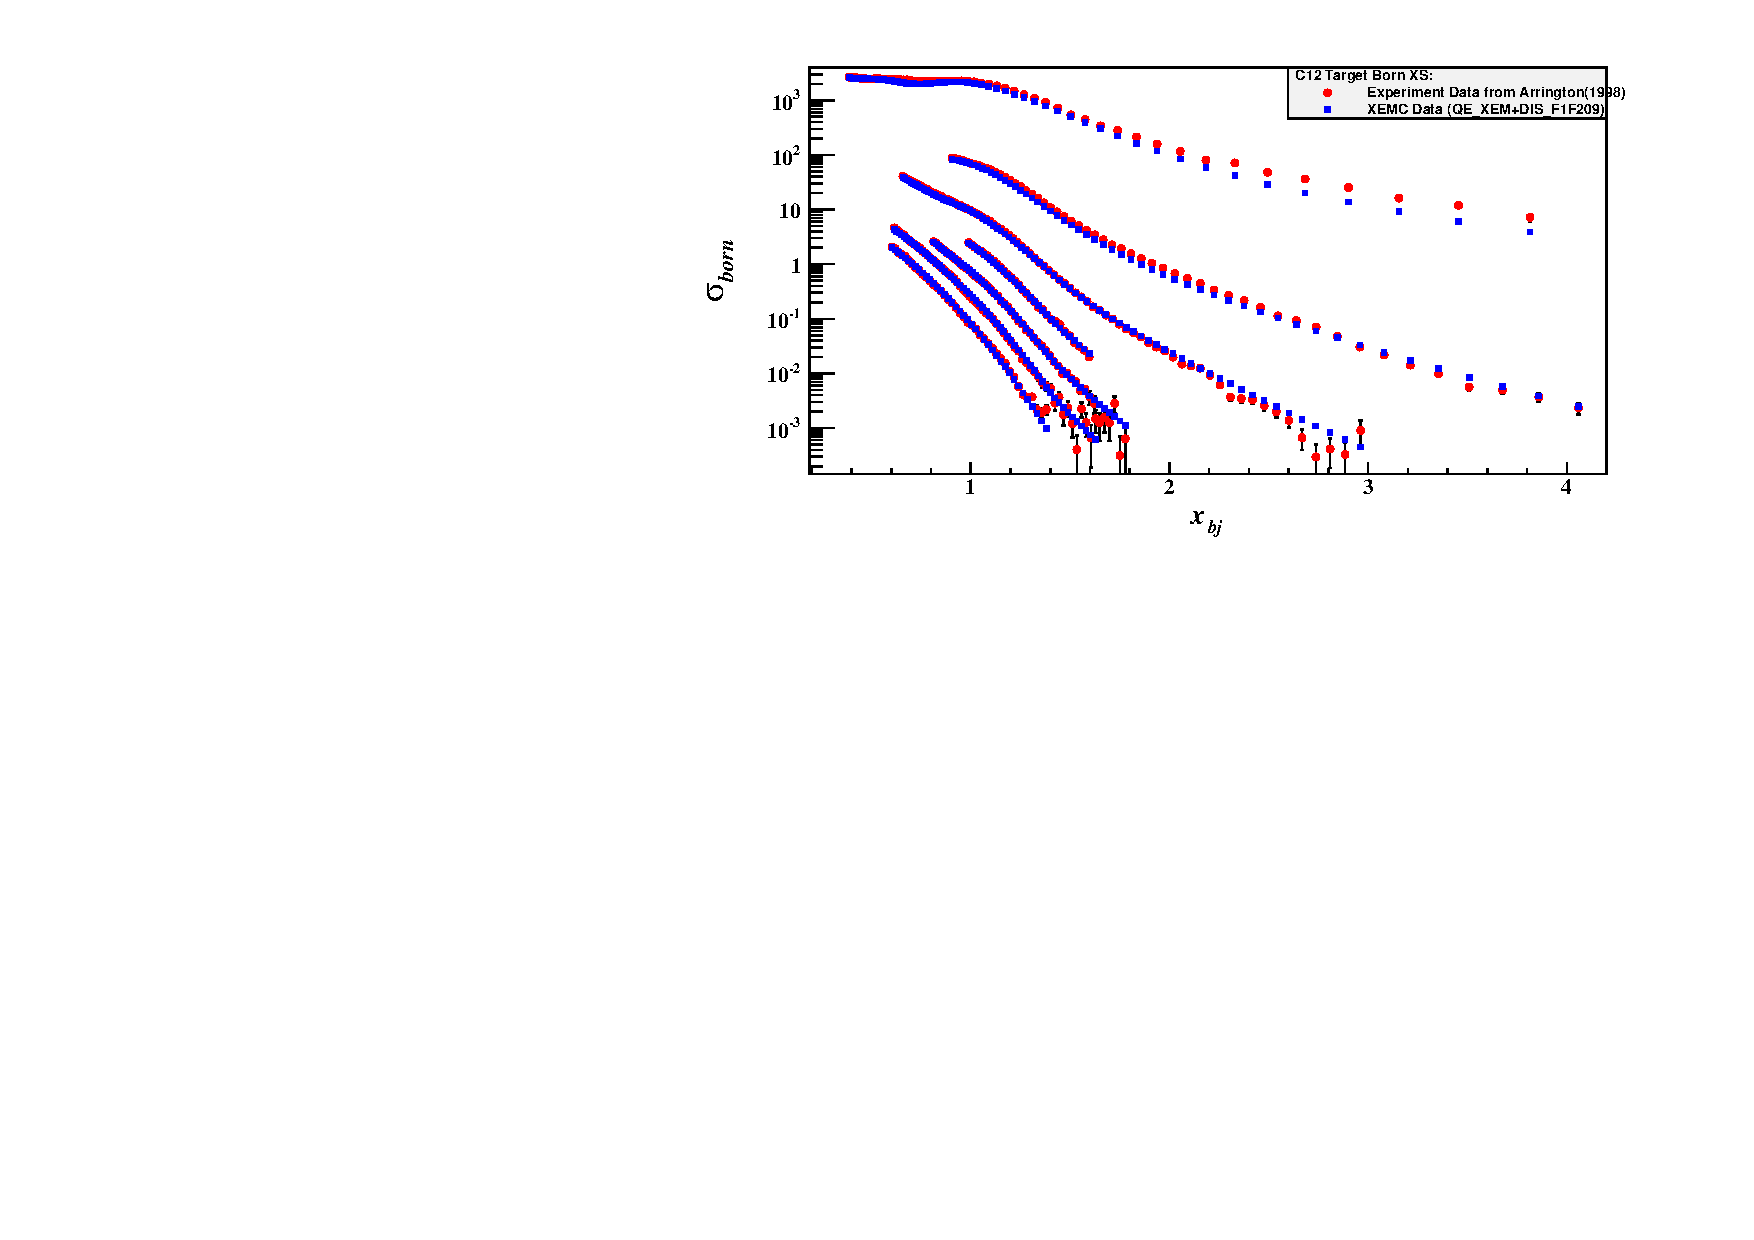
\includegraphics[type=pdf,ext=.pdf,read=.pdf,width=0.9\textwidth]{./figures/xemc/QEA_C12_Jan16_Born_Com_Arrington_1998}
    }
 \caption[Comparing XEMC models and experiment data for $\mathrm{^{4}He}$ and $\mathrm{^{12}C}$]{\footnotesize{Comparing XEMC models and experiment data for $\mathrm{^{4}He}$ and $\mathrm{^{12}C}$. Larger deviation can be seen in $\mathrm{^{12}C}$ data low $\mathrm{Q^{2}}$. Data is from QES-Archive~\cite{qe_donal}.}}   
  \label{xs_achieve_com2}
  \end{center}
\end{figure}
\begin{figure}[!h]
  \begin{center}
    \subfloat[$\mathrm{^{3}He}$ Born cross section]{
      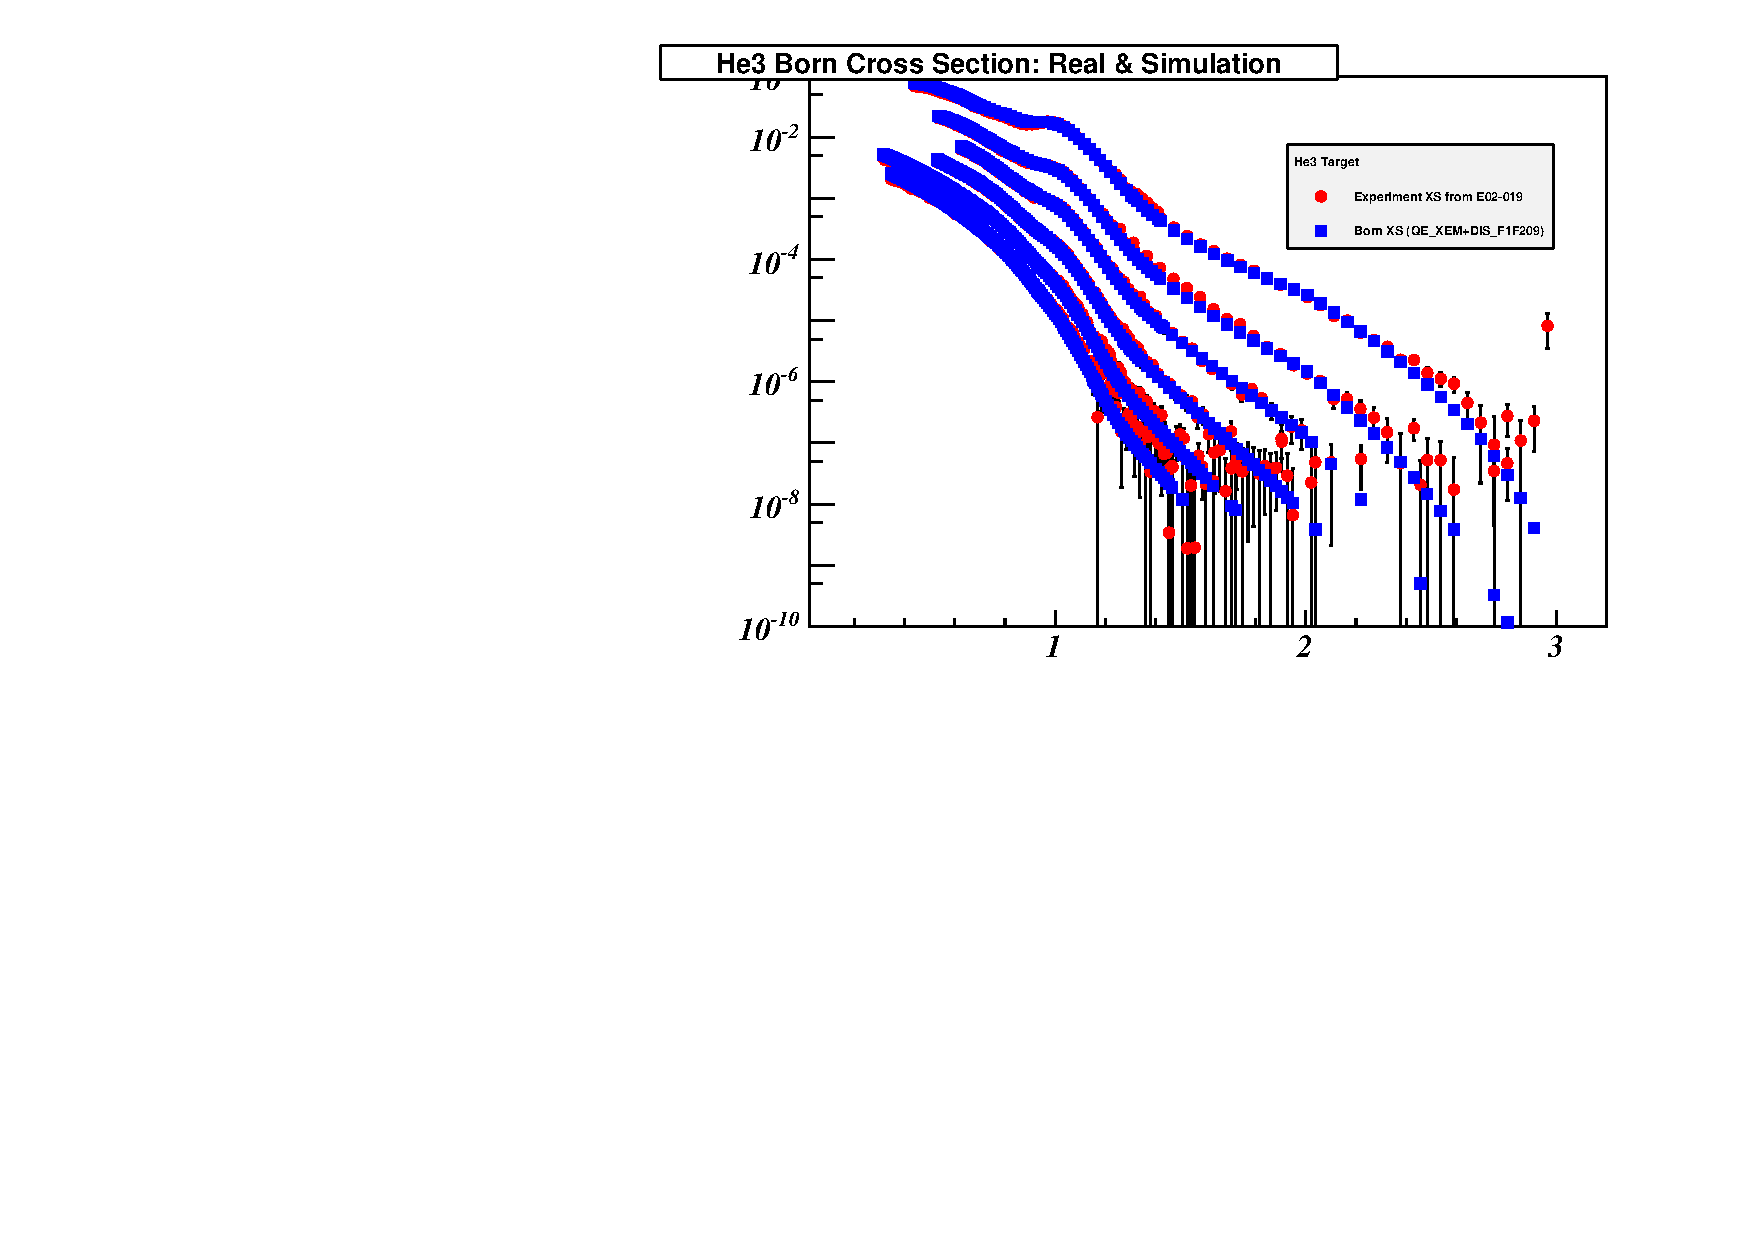
\includegraphics[type=pdf,ext=.pdf,read=.pdf,width=0.9\textwidth]{./figures/xemc/He3_XEMC_Born_Com}
      \label{xs_nadia_b1}
    }
    \\
       \subfloat[$\mathrm{^{3}He}$ radiated cross section]{
      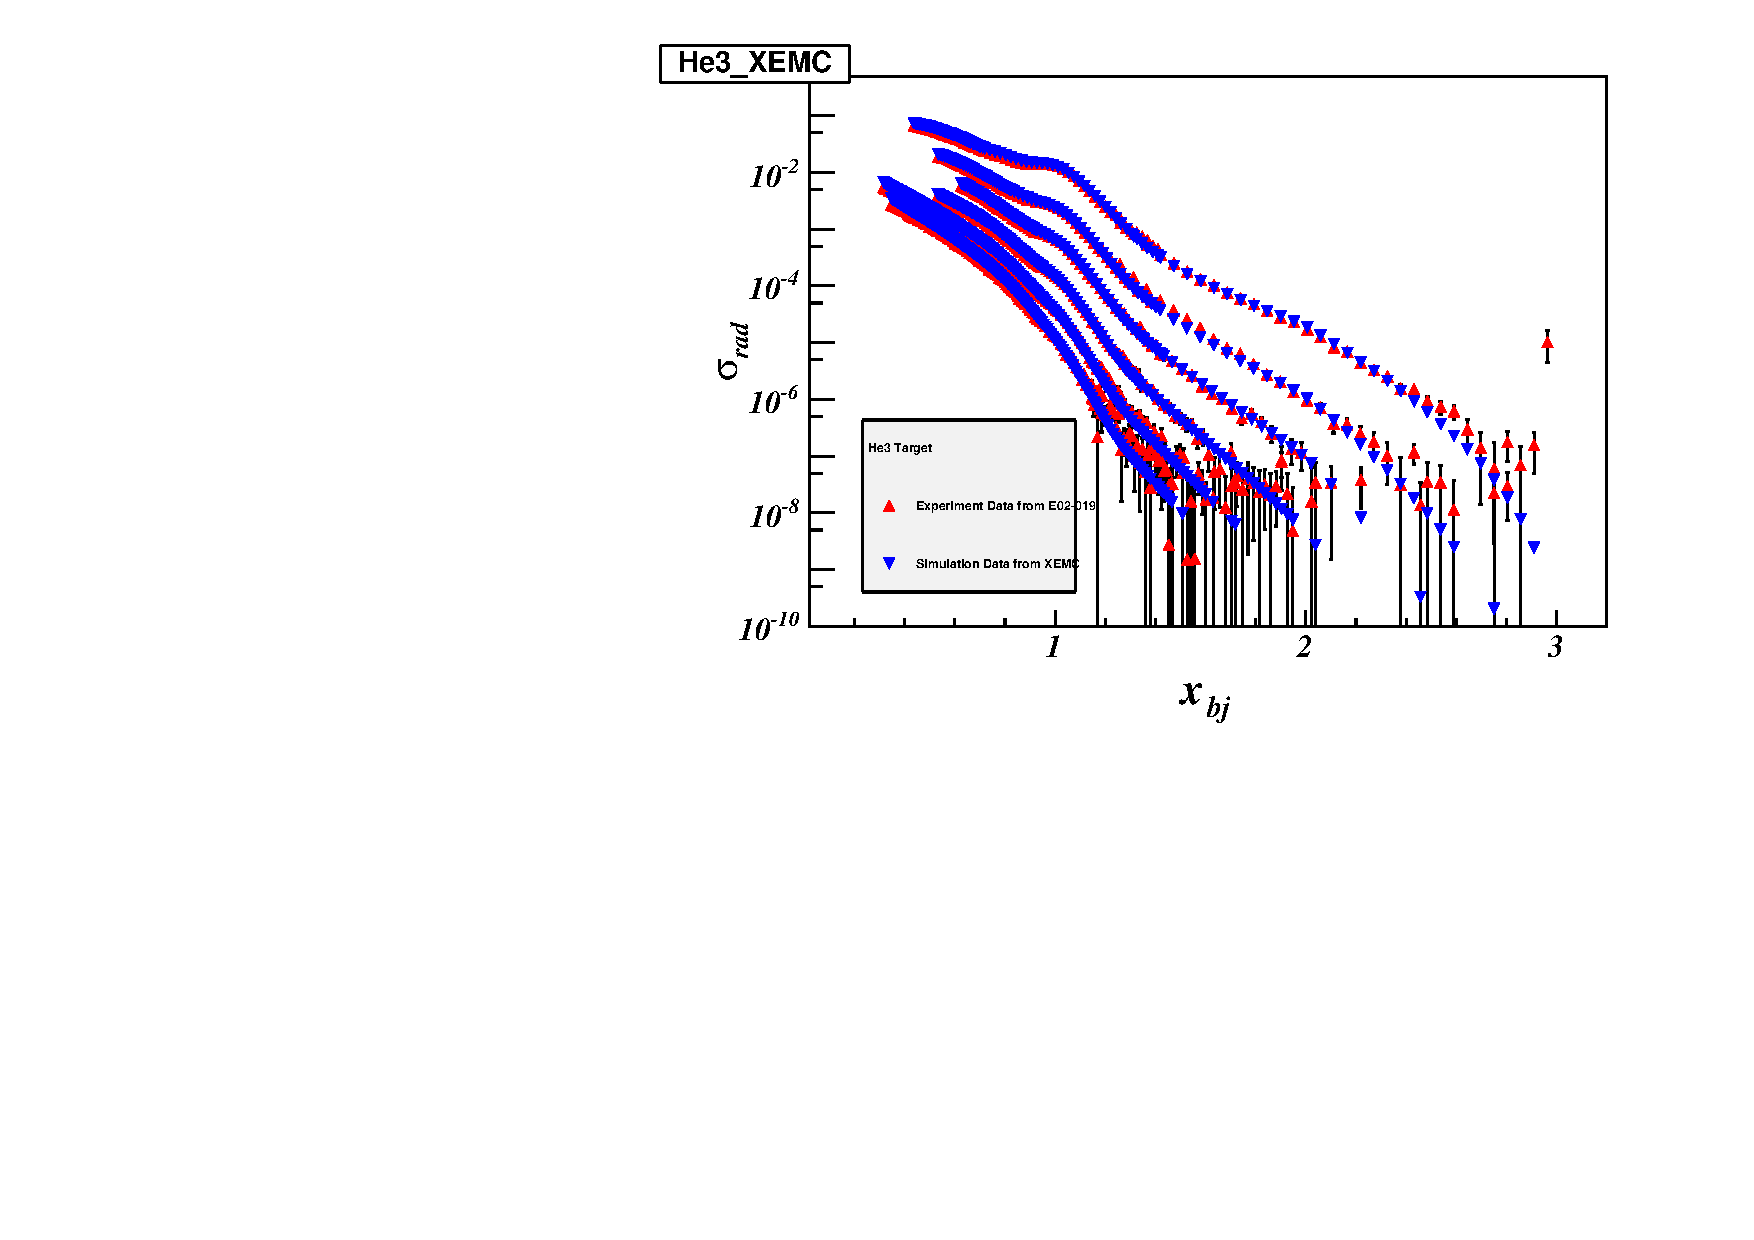
\includegraphics[type=pdf,ext=.pdf,read=.pdf,width=0.9\textwidth]{./figures/xemc/He3_XEMC_Rad_Com}
      \label{xs_nadia_r1}
    }
    \caption[Comparing $\mathrm{^{3}He}$ cross sections from E02-019 and calculated in XEMC]{\footnotesize{Comparing $\mathrm{^{3}He}$ cross sections from E02-019~\cite{nadia_thesis} and calculated in XEMC, where top and bottom plots are the Born and radiated cross section, respectively. The thickness of the target and the configuration of the target system are included~\cite{nadia_thesis}.}}
    \label{xs_nadia_com1}
  \end{center}
\end{figure}
\begin{figure}[!h]
  \begin{center}
     \subfloat[$\mathrm{^{12}C}$ Born cross section]{
      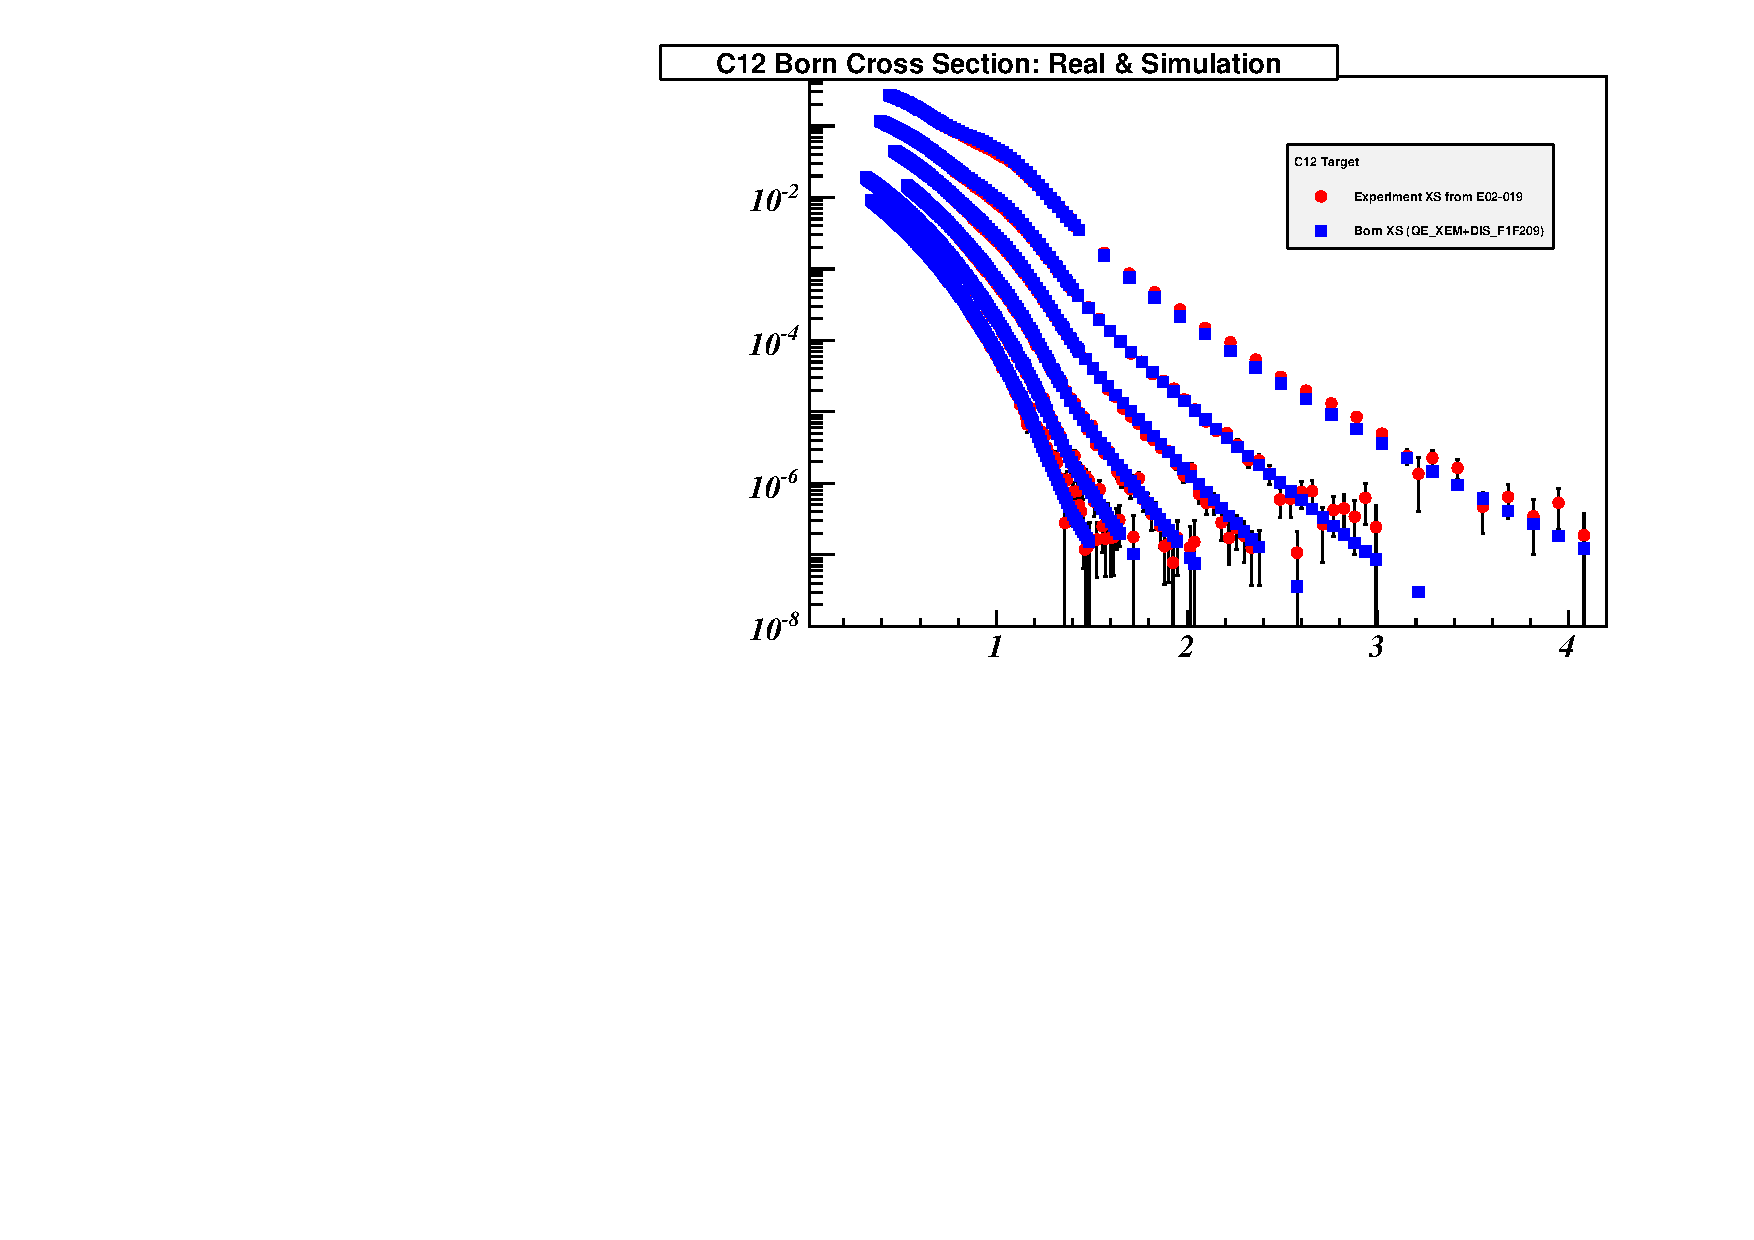
\includegraphics[type=pdf,ext=.pdf,read=.pdf,width=0.9\textwidth]{./figures/xemc/C12_XEMC_Born_Com}
      \label{xs_nadia_b2}
    }
    \\
     \subfloat[$\mathrm{^{12}C}$ radiated cross section]{
      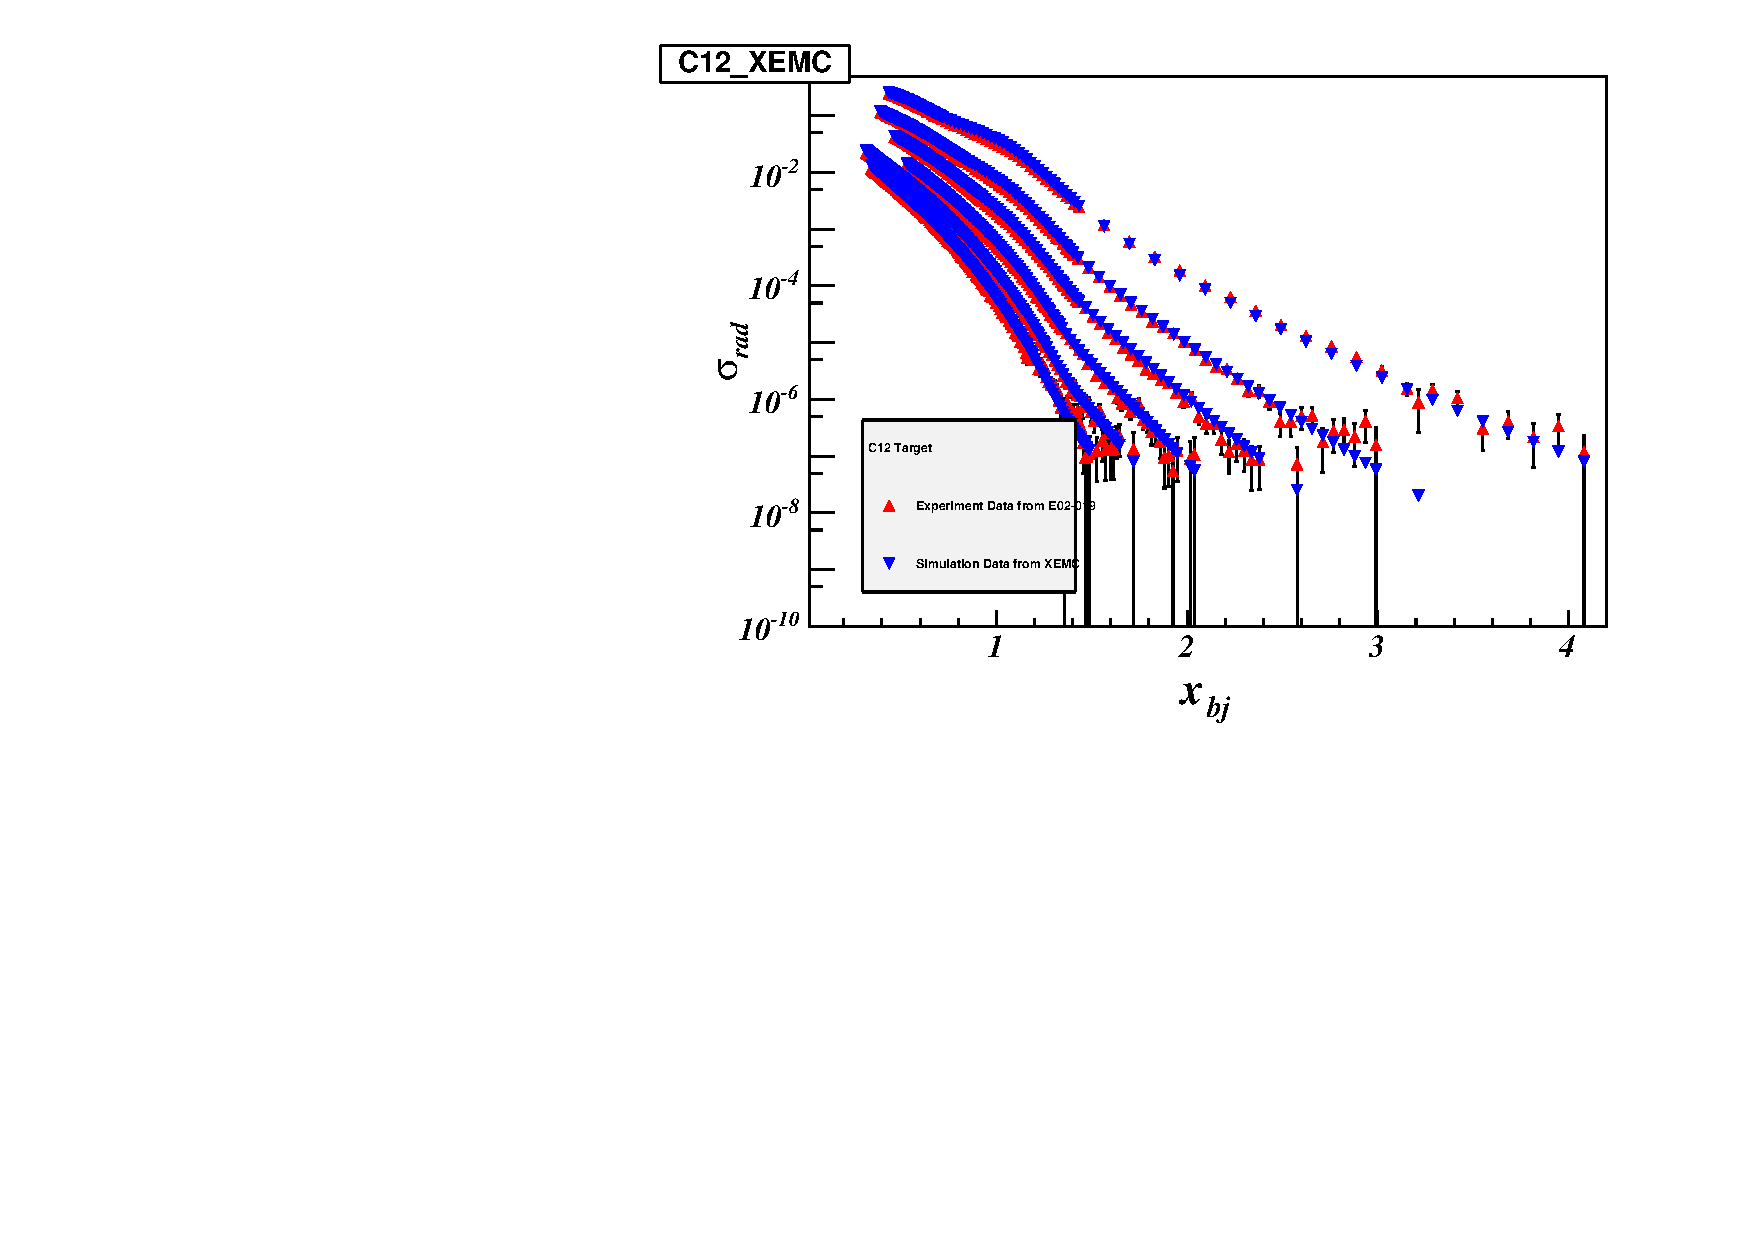
\includegraphics[type=pdf,ext=.pdf,read=.pdf,width=0.9\textwidth]{./figures/xemc/C12_XEMC_Rad_Com}
      \label{xs_nadia_r2}
    }
    \caption[Comparing $\mathrm{^{12}C}$ cross sections from E02-019 and calculated in XEMC]{\footnotesize{Comparing $\mathrm{^{12}C}$ cross sections from E02-019~\cite{nadia_thesis} and calculated in XEMC, where top and bottom plots are the Born and radiated cross section, respectively. The thickness of the target and the configuration of the target system are included~\cite{nadia_thesis}.}}
    \label{xs_nadia_com2}
  \end{center}
\end{figure}

\newpage
\section{Examples}
 An example to use the XEMC package is given in this section. 
% \newpage 
 \begin{lstlisting}
#include "XEMC.h"
int main(int argc,char** argv){
	XEMC* Event = new XEMC(); //Create a XEMC event
	//Target
	const int A = 12, Z = 6;    
	TString Target_Name = "C12";
    	Event->Init(Form("./input/%s_Input.dat",Target_Name.Data()));	
 	//Kinematic setting	
	double E0 = 3.356;    //GeV
	double Ep = 2.505;    //GeV/c
	double Theta = 25.00; //Degree
		
	//Calculate XS for the event
	int err = Event->Process(E0,Ep,Theta,A,Z);	
	if(err>=0){ //Return values
		double xs_rad  = Event->XS_Rad();
		double xs_qe   = Event->XS_QE();
		double xs_dis  = Event->XS_DIS();
		double xs_Born = Event->XS_Born();
	}
	//Print Out
	cerr<<Form("For %s Target, E0=%5.3f GeV, Ep=%5.3f GeV, Theta=%5.3f:",Target_Name.Data(), E0, Ep, Theta)<<endl;
	cerr<<Form("    XS_Born=%e, XS_QE=%e, XS_DIS=%e, XS_Rad=%e",
                    xs_Born, xs_qe, xs_dis, xs_rad)<<endl;	
	
	delete Event; //Release memory
}
\end{lstlisting}